% !TeX spellcheck = en_GB

\section{Background}

In order to explore the consequences of adding biological details to a neural system, we need to choose the desired computation that the neural system should ideally perform.
In machine learning, the simplest artificial neural networks are purely feed-forward, i.e., they possess no backwards-directed or \emph{recurrent} connections. It is well-known that feed-forward neural networks are universal function approximators \citep{hornik1989multilayer}.
That is, given enough neurons, any function $f(x) = y$ can be implemented as a neural network by simply having a single hidden layer of neurons that receives $x$ as an input (via a set of input weights) and produces $y$ as an output (via a set of readout weights).

Neurobiological systems differ from the artificial neural networks mentioned above in two key aspects.
First, they are intrinsically dynamical systems, i.e., input and output are functions over time.
Second, they often include recurrent connections.
As has been shown by \citet{eliasmith2003neural}, adding recurrent connections along with their associated synaptic dynamics allows for the creation of neural networks that approximate any differential equation of the form ${\mathrm{d}\vec m}/{\mathrm{d}t} = {\dot{\vec m}} = f(\vec m, u, t)$, where $f$ is an arbitrary function describing the dynamics, $\vec m$ is the system state, $u$ is an external input, and $t$ is time.
Again, with a sufficient number of neurons and the corresponding connectivity, such differential equations can be approximated to any desired degree of accuracy.
Our primary goal in this paper is to explore how well such computations can be performed in the presence of biological constraints. Once we have established this computational basis, we extend our network to a complete model of the eyeblink conditioning task and compare our simulation results to empirical data.

\subsection{The Legendre Delay Network}

As a benchmark for evaluating the impact of incorporating biological detail into a functional description, we choose the following linear differential equation $\theta\dot{\vec{m}} = \mat{A} \vec m + \mat{B} u$, where
\begin{align}	
    (\mat A)_{ij} &= \begin{cases}
        (2i + 1)(-1) & \text{if }i < j \,,\\
        (2i + 1)(-1)^{i - j + 1} & \text{if } i \geq j \,,
    \end{cases} &
    (\mat B)_i &= (2i + 1)(-1)^i \,.
    \label{eqn:delay_network_lti}
\end{align}
Here, $\vec m$ is a $q$-dimensional vector describing the current state of the linear system, $\mat A$ is a $q \times q$ matrix describing the state evolution, and $\mat B$ is a $q \times 1$ matrix describing how a scalar input $u$ influences the state.
This particular equation has been derived by taking the Padé approximants of the continuous-time delay $F(s)=e^{-\theta s}$ in the Laplace domain.
As such, this differential equation stores a compressed version of the past $\theta$ seconds of its inputs in the state variable $\vec m$ \citet{voelker2018improving}.
That is, given $\vec m$ at any point in time $t$, it is possible to recover an approximate value of $u$ at a previous point in time $\hat u(t - \theta')$ for $0 \leq \theta' \leq \theta$:
\begin{align}
	\hat u(t - \theta')
		&= \sum_{\ell = 0}^{q - 1} m_\ell d_\ell(\theta') \,, & \text{where } d_\ell(\theta') &= \tilde P_\ell \left(\frac{\theta'}{\theta}\right)
		= 
(-1)^\ell \sum_{k = 0}^\ell \binom{\ell}k \binom{\ell + k}k
			\left(-\frac{\theta'}{\theta}\right)^k\,.
	\label{eqn:delay_network_decoder}
\end{align}
The function $\tilde P_\ell$ is the shifted Legendre polynomial of degree $\ell$.

Another way to think of this system is that it encodes the past history of its inputs using a set of \textit{temporal basis functions}. The temporal basis functions that happen to form the representational basis of the above linear system are the Legendre polynomials $\tilde P_\ell$, which have been shown to be optimal for encoding such temporal memory \cite{voelker2018improving}.
Of course, some information is lost in this process of compressing the history of $u$ into $\vec m$. The quality with which past $u$ can be reconstructed from $\vec m$ is controlled by the number of state dimensions $q$, or, more precisely, the ratio of $q$ and $\theta$.
As $q$ increases for a constant $\theta$, more details (i.e., higher frequencies) about the past are represented in $\vec m$.

The neural implementation of this computation is called a \enquote{Legendre Delay Network}~(LDN).
Crucially, arbitrary functions over the time interval $[t - \theta, t]$ can be decoded from the neurons representing the network state $\vec m$, and not just delays. In other words, the LDN forms the filter bank of an adaptive filter, a hypothesized functional description of the Granule-Golgi circuit in the cerebellum \citet{fujita1982adaptive}. The LDN has previously been used to model cognitive timing behavior in humans \citet{jong2019flexible} and is also the core component of a novel machine learning algorithm known as the Legendre Memory Unit~(LMU), which has been shown to outperform LSTMs on several benchmark tasks \citep{voelker2019lmu}.

If we use biologically constrained neural networks to approximate the above linear system, then the actual computation performed by the system, and hence the quality of the time window encoded in $\vec m$, may be different.
We can thus use this system as a benchmark.
In the following, after discussing the cerebellum in more detail, we build various approximations of the LDN using different biological constraints, systematically provide them with inputs, and evaluate their performance in terms of how well the input history can be recovered. Finally, we integrate the LDN into a model of the cerebellum performing the eyeblink conditioning task.
To create the model, we compute optimal input and recurrent connection weights independently for each target population to approximate functional descriptions such as \cref{eqn:delay_network_lti} given biological constraints.
This means we are not modelling the entire developmental process for the cerebellum, but are rather directly creating a model of a mature cerebellum.  For the full eyeblink conditioning task, we then also apply a local biologically plausible learning rule to learn the readout weights.

\subsection{Eyeblink Conditioning}

The cerebellum is well-studied and highly regular in its structure, and there are reasons to believe that the cerebellum does compute something akin to the operation performed by the Legendre Delay Network \citet{fujita1982adaptive}. Behaviourally, the cerebellum is known to be vital for some delay conditioning tasks, such as eyeblink conditioning.

In eyeblink conditioning, a puff of air is directed at the eye (unconditioned stimulus; US), triggering the eyeblink reflex (unconditioned response; UR). The US is paired with a neutral, conditioned stimulus (CS), for example a short tone. The CS precedes the US by a constant time offset $\Delta t$. Over time the subject forms a conditioned response (CR) to the previously neutral CS, maintaining the fixed delay $\Delta t$. In other words, the subject will learn to have its eye closed $\Delta t$ seconds after the tone, even if the puff is absent \citep[cf.][]{heiney2014cerebellardependent}. Experiments indicate that the formation of this conditioned response critically depends on the cerebellum; previously learned CRs are absent once the cerebellum is ablated \citep{mccormick1981engram}.

\subsection{Cerebellar Microcircuitry}

\begin{figure}[t]
	\centering
	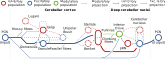
\includegraphics[scale=0.95]{media/chapters/05_cerebellum/cerebellum_anatomy.pdf}
	\caption[Schematic of the cerebellar microcircuit.]{Schematic of the cerebellar microcircuit. Dashed projections and populations are not included in our model. Cerebellar nucleus afferents affect both the excitatory and inhibitory sub-populations.  The main feed-forward pathway is highlighted in bold. \emph{PCN}~$\hat=$~pre-cerebellar neurons/nuclei. \emph{pRN}~$\hat=$~parvicellular Red Nucleus. Data from \citet{ito2010cerebellar,llinas2010olivocerebellar}.}
	\label{fig:cerebellum_anatomy}
\end{figure}

Before we continue to discuss the two prevalent theories on how the cerebellum could learn the conditioned response, it is worthwhile to review the cerebellar microcircuitry depicted in Fig.~\ref{fig:cerebellum_anatomy}.
Afferent nerves from pre-cerebellar (PC) nuclei (brainstem and cerebral cortex carrying sensory signals) project as \enquote{mossy fibers} onto granule cells in the cerebellar cortex.
Cerebellar granule cells are tiny and account for the majority of neurons in the mammalian brain. Thus, very few PC neurons connect onto a very large number of granule cells.

Granule cells also have inter-neurons interspersed amongst them, known as Golgi cells, forming an inhibitory feedback loop with the granule cells. That is, granule cells excite Golgi cells, and Golgi cells inhibit granule cells \citep{ito2010cerebellar}.
Notably, the connections from Golgi and PC cells to granule cells are formed through so called glomeruli. Each granule cells extends to on average four glomeruli and, at each glomerulus, receives input from one PC neuron through a mossy fiber terminal, as well as one or more Golgi cells \citep{palkovits1972quantitative,jakab1988quantitative,chadderton2004integration}.
Furthermore, the connectivity between Golgi and granule cells is spatially constrained, i.e., Golgi cells only connect to granule cells in their vicinity \citep{dangelo2013cerebellar}. The ratio of granule to Golgi cells is about 400:1 \citep{korbo1993total}.

Granule cell axons, the so called \enquote{parallel fibers,} project onto the Purkinje cells, which inhibit neurons in the cerebellar nucleus, and in turn project back onto the brainstem and cerebral cortex \citep{ito2010cerebellar,llinas2010olivocerebellar}. So called \enquote{climbing fibers} project from Inferior Olive neurons in the deep cerebellar nucleus onto Purkinje cells. 
Evidence suggests that activity in the climbing fibers is responsible for modulating the synaptic strength of granule to Purkinje projections. Climbing fiber activity can thus be interpreted as an \enquote{error signal} responsible for driving learning in the cerebellar cortex \citep{ito2010cerebellar}.

\subsection{Hypothesized Mechanisms Supporting Delay Learning}

There is no current consensus on what the exact mechanism is that supports delay learning in the cerebellum.
The classical view is the aforementioned adaptive filter theory \citep{fujita1982adaptive}.
As originally pointed out by \citep{marr1969theory}, the massive divergence (number of post-neurons for a single pre-neuron) and small convergence (number of pre-neurons for a single post-neuron) in the PC to granule projection suggests that granular cells are tuned to specific patterns of activity in the PC neurons.
The adaptive filter theory can be interpreted as extending this idea toward temporal tuning.
Granule cell activity does not only depend on the current PC activities, but on their time-course. Such a temporal tuning could be the result of the recurrent granule-to-granule connections mediated by the inhibitory Golgi cells.
If this temporal tuning is diverse enough, i.e., granule cells are sensitive to different time-courses, this will form a suitable temporal basis from which arbitrary delays can be decoded.
Learning a specific decoding is driven by the climbing fiber error signal, modulating the synaptic weights between the granule and the Purkinje cells.
As mentioned above, this is similar in principle to the Legendre Delay Network.

A more recent theory is that responses observed in tasks such as eyeblink conditioning inherently rely on intrinsic properties of the Purkinje cells.
In other words, temporal properties of the granule cells play a lesser role.
Instead, climbing fiber input triggers processes within the Purkinje cell and their dendritic structures that are responsible for the formation of a delayed output.
Indeed, \citet{johansson2014memory} find that bypassing the granule cells and directly injecting signals into the parallel fibers still evokes a previously learned delayed response from the cerebellum, albeit a weaker one.

We think that these two theories are not inherently contradictory. Both temporal tuning of the granular cells and intrinsic temporal properties of the Purkinje cells could play a role in delay learning.
The findings we present in this paper provide a strong argument that the biology of the Granule-Golgi circuit is at least well suited for implementing some kind of temporal basis function generation, and as such confirms the results of previous studies  \citep[cf.][]{dean2010cerebellar,rossert2015edge}.
Still, our work only takes a fraction of the available data on cerebellar neurophysiology into account and as such should not be seen as strong evidence for or against one of the two proposed mechanisms.
Instead, we are interested in describing methods for adding biological constraints while determining their consequences for higher-level function.
